\section{Resultados para o nosso caso}
\label{sec:ik_resultados}

\subsection{Exemplo 1: alvo com a garra na vertical}

Tomou-se o ponto $(x, y, z) = (0;\ 0{,}20;\ 0{,}06)$~m, no referencial da base, com $\psi = 90^\circ$, isto é, $\alpha_3 = -90^\circ$. Pelas Equações~\eqref{eq:ik_d} a~\eqref{eq:ik_beta}:
\begin{align*}
    r &= 0{,}2000~\mathrm{m}, \qquad d = \sqrt{0{,}2^2 - 0{,}0646^2} = 0{,}1893~\mathrm{m}\\
    q_1 &= 90^\circ - \operatorname{atan2}(0{,}1893;\ 0{,}0646) = 90^\circ - 71{,}16^\circ = 18{,}84^\circ\\
    x_{3d} &= 0{,}1893 - 0{,}0731 = 0{,}1162~\mathrm{m}\\
    y_{3d} &= (0{,}06 - 0{,}1316) + 0{,}1513 = 0{,}0797~\mathrm{m}\\
    r_3 &= 0{,}1409~\mathrm{m}, \qquad \alpha_1 = 34{,}45^\circ, \qquad \beta_1 = 42{,}81^\circ, \qquad \beta_2 = 85{,}79^\circ
\end{align*}

Com o cotovelo para cima, $\theta_1 = \alpha_1 + \beta_1 = 77{,}26^\circ$ e $\theta_2 = -(180^\circ - \beta_2) = -94{,}21^\circ$; o cotovelo fica a 0,239~m de altura, contra 0,116~m na solução de cotovelo para baixo. Pelas Equações~\eqref{eq:ik_theta3} e~\eqref{eq:ik_q234}, $q_2 = -12{,}74^\circ$, $q_3 = -94{,}21^\circ$ e $q_4 = 0^\circ - 77{,}26^\circ + 94{,}21^\circ = 16{,}95^\circ$. O resultado foi
\begin{equation*}
    \mathbf{q} = (18{,}84^\circ;\ -12{,}74^\circ;\ -94{,}21^\circ;\ 16{,}95^\circ;\ 0^\circ;\ 0^\circ)
\end{equation*}

É a configuração de trabalho usada na verificação da cinemática direta (Equação~\ref{eq:q_trabalho}), que devolveu exatamente o alvo, $(0;\ 0{,}2000;\ 0{,}0600)$~m, com a garra a apontar para baixo. Isto fecha o ciclo entre as duas cinemáticas.

\subsection{Exemplo 2: alvo longe, que obriga a inclinar a garra}

Tomou-se agora $(x, y, z) = (0{,}05;\ 0{,}30;\ 0{,}02)$~m. Aqui, $r = 0{,}3041$~m, $d = 0{,}2972$~m e $z - L_1 = -0{,}1116$~m. Com $\psi = 90^\circ$, $x_{3d} = 0{,}2241$~m e $y_{3d} = 0{,}0397$~m, ou seja, o pulso ficaria a $r_3 = 0{,}2276$~m do ombro, acima do máximo $L_2 + L_3 = 0{,}2064$~m: o argumento de $\beta_2$ vale $-1{,}434$, fora de $[-1, 1]$, e não há solução.

Como o alvo está longe, inclinar a garra para a base afasta ainda mais o pulso, pelo que só funcionam inclinações $\psi < 90^\circ$. A procura parou em $\psi \approx 82{,}27^\circ$, onde $r_3 \approx L_2 + L_3$ e o braço fica quase esticado, o que mostra que o ponto está no limite do alcance. Os ângulos foram
\begin{equation*}
    \mathbf{q} = (2{,}80^\circ;\ -81{,}96^\circ;\ -0{,}21^\circ;\ -0{,}10^\circ;\ 0^\circ;\ 0^\circ)
\end{equation*}
e a cinemática direta devolveu $(0{,}05;\ 0{,}30;\ 0{,}02)$~m, com a garra a apontar para $(-0{,}0066;\ 0{,}1343;\ -0{,}9909)$: para baixo, ligeiramente para fora.

\begin{figure}[H]
  \centering
  \resizebox{0.9\textwidth}{!}{% Poses calculadas nos dois exemplos da cinemática inversa (plano do braço); unidades em cm
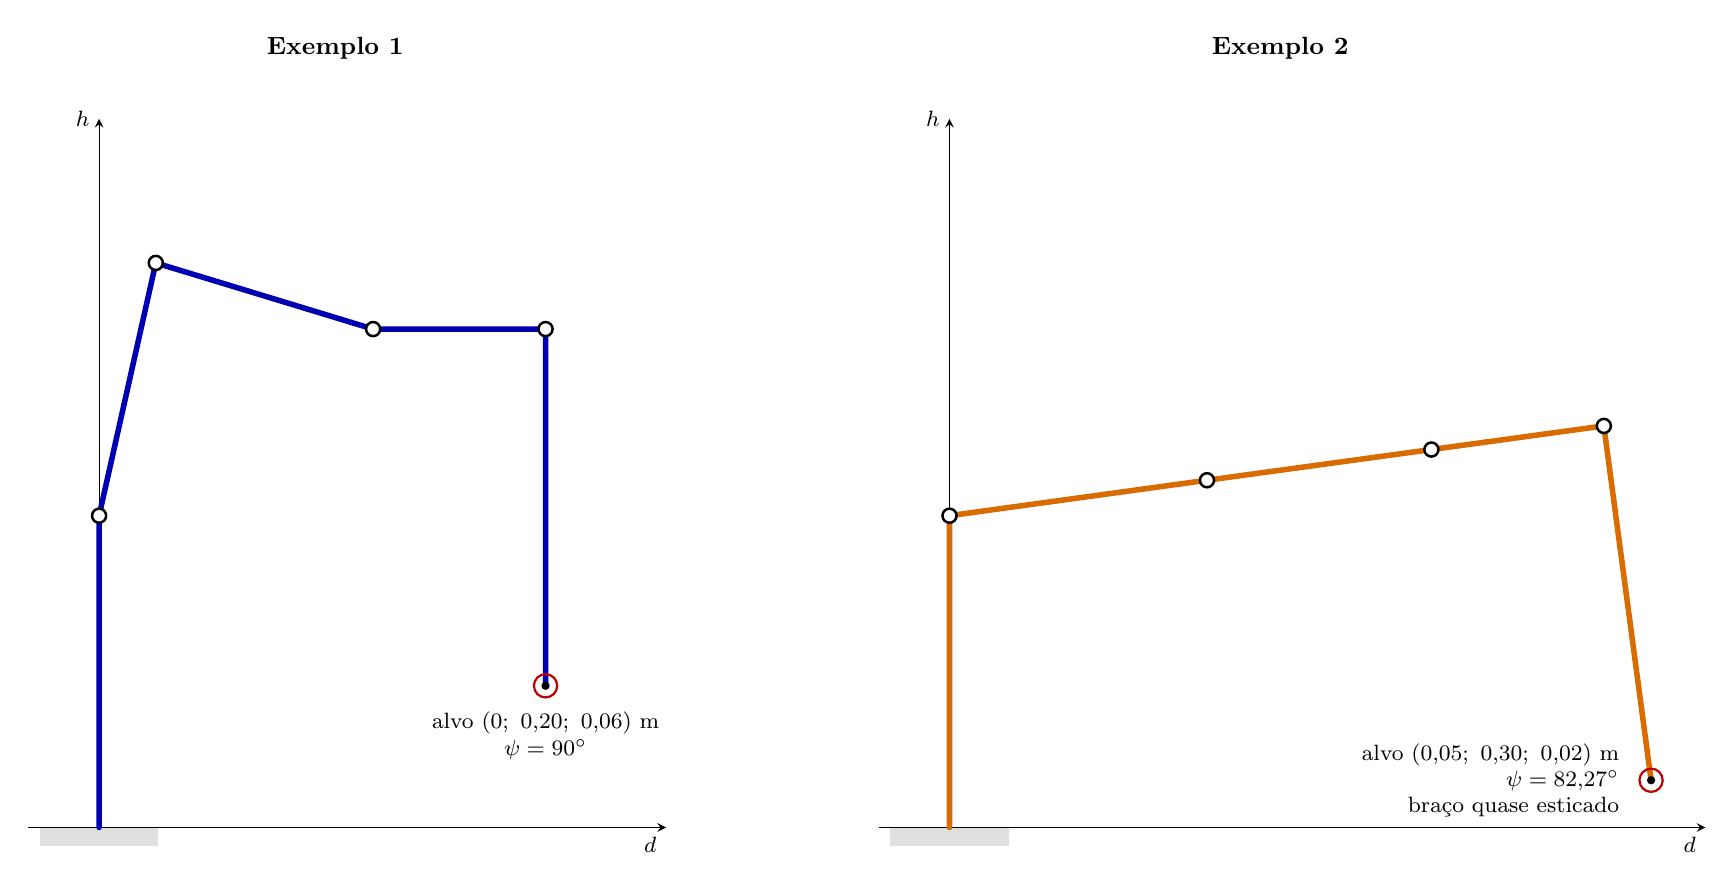
\begin{tikzpicture}[scale=0.3, >=stealth,
    elo/.style={line width=2pt, line cap=round},
    junta/.style={circle, draw, fill=white, line width=0.9pt, inner sep=1.8pt},
    cota/.style={gray!70!black, thin},
    ang/.style={->, thin},
    every node/.style={font=\footnotesize}]

  \draw[->, thin] (-3,0) -- (24,0) node[below left] {$d$};
  \draw[->, thin] (0,0) -- (0,30) node[left] {$h$};
  \fill[gray!25] (-2.5,-0.8) rectangle (2.5,0.0);
  \draw[elo, blue!70!black] (0.0,0.0) -- (0.0,13.2) -- (2.4,23.9) -- (11.6,21.1) -- (18.9,21.1) -- (18.9,6.0);
  \node[junta] at (0.0,13.2) {};
  \node[junta] at (2.4,23.9) {};
  \node[junta] at (11.6,21.1) {};
  \node[junta] at (18.9,21.1) {};
  \fill (18.9,6.0) circle (5pt);
  \draw[red!75!black, thick] (18.9,6.0) circle (14pt);
  \node[below=6pt, align=center] at (18.9,6.0) {alvo $(0;\ 0{,}20;\ 0{,}06)$ m\\$\psi = 90^\circ$};
  \node[font=\small\bfseries] at (10,33) {Exemplo 1};
  \draw[->, thin] (33,0) -- (68,0) node[below left] {$d$};
  \draw[->, thin] (36,0) -- (36,30) node[left] {$h$};
  \fill[gray!25] (33.5,-0.8) rectangle (38.5,0.0);
  \draw[elo, orange!85!black] (36.0,0.0) -- (36.0,13.2) -- (46.9,14.7) -- (56.4,16.0) -- (63.7,17.0) -- (65.7,2.0);
  \node[junta] at (36.0,13.2) {};
  \node[junta] at (46.9,14.7) {};
  \node[junta] at (56.4,16.0) {};
  \node[junta] at (63.7,17.0) {};
  \fill (65.7,2.0) circle (5pt);
  \draw[red!75!black, thick] (65.7,2.0) circle (14pt);
  \node[left=8pt, align=right] at (65.7,2.0) {alvo $(0{,}05;\ 0{,}30;\ 0{,}02)$ m\\$\psi = 82{,}27^\circ$\\braço quase esticado};
  \node[font=\small\bfseries] at (50,33) {Exemplo 2};
\end{tikzpicture}}
  \caption{Poses obtidas pela cinemática inversa nos dois exemplos, no plano do braço.}
  \label{fig:exemplos_ik}
\end{figure}

Nos dois casos, a cinemática direta devolveu o ponto pedido, o que valida a cinemática inversa.

\clearpage